% Guide : Lancement d’un script Python pour entraînement ou test de réseau de neurones sur le cluster Curta (MCIA) avec GPU
\documentclass[a4paper,12pt]{article}
\usepackage[utf8]{inputenc}
\usepackage[T1]{fontenc}
\usepackage[french]{babel}
\usepackage{xcolor}
\usepackage{tcolorbox}
\tcbuselibrary{skins,breakable,listings}
\usepackage{graphicx}
\usepackage{hyperref}
\usepackage{listings}
\usepackage{sectsty} % Pour colorer les titres

% Définition des couleurs
\definecolor{cmdbg}{RGB}{255,250,205}    % jaune clair
\definecolor{cmdfg}{RGB}{0,0,0}          % texte noir
\definecolor{sectioncolor}{RGB}{0,102,204}   % bleu pour sections
\definecolor{subsectioncolor}{RGB}{204,102,0} % orange pour sous-sections

% Appliquer la couleur aux titres
\sectionfont{\color{sectioncolor}}
\subsectionfont{\color{subsectioncolor}}

% Configuration des boîtes de commandes (terminal)
\newtcolorbox{terminal}[1][]{%
  colback=cmdbg, colframe=black, coltext=cmdfg,
  boxrule=0.5pt, arc=2pt, outer arc=2pt,
  enhanced, breakable,
  fontupper=\ttfamily\small,
  title=#1
}

% Configuration des listings pour code Python
\lstset{
  basicstyle=\color{cmdfg}\ttfamily\small,
  backgroundcolor=\color{cmdbg},
  keywordstyle=\color{blue},
  commentstyle=\color{gray},
  stringstyle=\color{olive},
  frame=single,
  rulecolor=\color{black},
  breaklines=true,
  showstringspaces=false,
}

\title{Guide : Lancement d’un script Python pour \textbf{entraînement} ou \textbf{test} de réseau de neurones sur le cluster \textit{Curta} (MCIA) avec GPU}
\author{Oussama Guelfaa (@guelfaao)}
\date{23 juin 2025}

\begin{document}
\maketitle

\tableofcontents
\newpage

\section{Introduction}
Ce guide décrit étape par étape comment :
\begin{itemize}
\item Transférer votre code et vos données vers le cluster MCIA (Curta),
\item Se connecter via Open OnDemand,
\item Charger les modules nécessaires (GPU, Python, CUDA),
\item Lancer votre script Python d’entraînement ou de test de réseau de neurones,
\item Surveiller et récupérer les résultats.
\end{itemize}

\section{Prérequis}
\begin{itemize}
\item Compte utilisateur sur \texttt{curta.mcia.fr} (identifiant \texttt{guelfaa}).
\item Fichier \texttt{Inversion\_anneaux.zip} contenant votre projet.
\item Accès au portail Open OnDemand de MCIA.
\item Modules disponibles : Python, CUDA, cuDNN, TensorFlow/PyTorch.
\end{itemize}

\section{1. Transfert des fichiers (SCP)}
Le transfert de vos fichiers vers le cluster est essentiel pour exécuter vos scripts sur les ressources distantes. Nous utilisons \texttt{scp} (Secure Copy) pour copier votre archive :

\begin{terminal}[Transfert du ZIP]
(base) MacBook-Pro-de-Oussama:~ oussamaguelfaa\$ scp “/Users/oussamaguelfaa/Desktop/Stage/Inversion\_anneaux.zip” \
guelfaa@curta.mcia.fr:~
\end{terminal}

Il vous sera demandé votre mot de passe :
\begin{terminal}[Invite de mot de passe]
guelfaa@curta.mcia.fr’s password:
\end{terminal}

Une barre de progression vous informe de l’avancement du transfert.
Après quelques instants, le transfert se termine :
\begin{terminal}[Progression du transfert]
Inversion\_anneaux.zip \hfill 9\%   90MB  13.1MB/s   01:07 ETA
\end{terminal}

\section{2. Connexion via OpenOnDemand}
Accédez au portail web : \url{https://curta3.mcia.fr/pun/sys/dashboard} (ou votre URL de l’instance MCIA).
Open OnDemand offre une interface web pour accéder aux ressources du cluster sans SSH direct.

\begin{figure}[h!]
  \centering
  % Capture d'écran du portail OpenOnDemand
  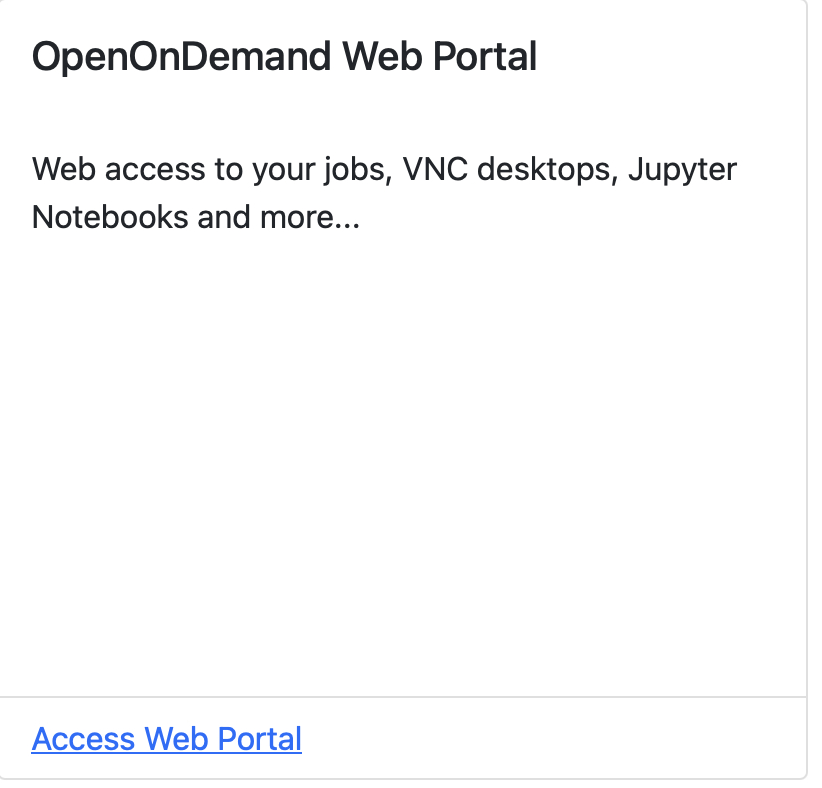
\includegraphics[width=0.8\textwidth]{OnDemandPortam.png}
  \caption{Portail OpenOnDemand MCIA}
  \label{fig:openondemand}
\end{figure}

Une fois connecté, dans la barre de menu :
\begin{enumerate}
\item Cliquez sur \textbf{Apps} (coin supérieur gauche).
\item \textbf{All Apps} puis \textbf{Curta Shell Access}.
\end{enumerate}

Vous serez redirigé vers une invite de terminal web :
\begin{terminal}[Ouverture du shell]
guelfaa@curta.mcia.fr's password:
Last login: Fri Jun 20 16:10:06 2025 from 147.210.55.176

Use the following commands to adjust your environment:

'module avail'            – show available modules  
'module add <module>'     – adds a module to your environment for this session  
'module initadd <module>' – configure module to be loaded at every login

Disk quotas for user guelfaa (uid 130068):
                          Block Limits                     File Limits


[guelfaa@login02 ~]\$ ls
\end{terminal}

\section{3. Préparation de l’environnement}
Avant de lancer vos scripts, il est crucial de charger les bons modules afin d’avoir accès au GPU, à Python et aux bibliothèques ML.

\subsection{3.1. Liste des modules disponibles}
Afficher tous les modules installés :
\begin{terminal}[module avail]
module avail
\end{terminal}

\subsection{3.2. Chargement des modules GPU et Python}
Par exemple, pour charger CUDA et Python 3.9 :
\begin{terminal}[Chargement des modules]
module add cuda/11.7
module add python/3.9
\end{terminal}

Vous pouvez vérifier les modules chargés :
\begin{terminal}[module list]
module list
\end{terminal}

\section{4. Décompression et exécution du script}

\subsection{4.1. Décompression du projet}
\begin{terminal}[Décompression]
unzip Inversion\_anneaux.zip -d Inversion\_anneaux
cd Inversion\_anneaux
\end{terminal}

\subsection{4.2. Lancement de l’entraînement (exemple Slurm)}
Une fois les modules prêts, préparez votre projet et lancez le job via le système d’ordonnancement Slurm.
Si vous utilisez Slurm : créez un script \texttt{train.sh} :

\begin{lstlisting}[caption=Exemple de script Slurm (train.sh)]
#!/bin/bash
#SBATCH --job-name=train_nn
#SBATCH --gres=gpu:1               # demande un GPU
#SBATCH --cpus-per-task=4          # coeurs CPU
#SBATCH --mem=16G                  # memoire RAM
#SBATCH --time=02:00:00            # duree max
#SBATCH --output=out_%j.log        # fichier de sortie

module add cuda/11.7
module add python/3.9

python train.py --config config.yaml
\end{lstlisting}

Puis soumettez le job :
\begin{terminal}[Soumission du job]
sbatch train.sh
\end{terminal}



Après soumission du job, vous pouvez suivre l'état de votre job lorsqu'il est en file d'attente ou en cours d'exécution en utilisant la commande \texttt{squeue}. Cette commande liste tous vos jobs actifs sur le cluster.

\begin{terminal}[Suivi du job]
squeue -u guelfaa
\end{terminal}

Par exemple, la sortie peut ressembler à :

\begin{terminal}[Exemple de sortie \texttt{squeue}]
JOBID   PARTITION  NAME      USER     ST       TIME  NODES NODELIST(REASON)\\
123456  gpu        train\_nn  guelfaa  R    00:10:23     1    node05\\
123457  gpu        train\_nn  guelfaa  PD   00:00:00     1    (Priority)
\end{terminal}

\subsection{4.3. Lancement du test}
Adaptez le script :
\begin{lstlisting}[caption=Exemple de script Slurm (test.sh)]
#!/bin/bash
#SBATCH -job-name=test_nn
#SBATCH -gres=gpu:1
#SBATCH -cpus-per-task=2
#SBATCH -mem=8G
#SBATCH -time=01:00:00
#SBATCH -output=test_%j.log

module add cuda/11.7
module add python/3.9

python test.py -model model_best.pth
\end{lstlisting}

Soumission :
\begin{terminal}[Soumission du test]
sbatch test.sh
\end{terminal}

\section{5. Suivi et récupération des résultats}

Après exécution, les logs sont disponibles :
\begin{terminal}[Visualisation du log]
less out\_.log
\end{terminal}

Pour récupérer vos résultats :
\begin{terminal}[Récupération via SCP]
scp guelfaa@curta.mcia.fr:~/Inversion\_anneaux/results/*.png ./results/
\end{terminal}

\section{Conclusion}
Ce guide vous permet de transférer, lancer et suivre vos scripts Python de réseaux de neurones sur le cluster Curta avec GPU.\newline


\end{document}
